\documentclass{article}\usepackage[]{graphicx}\usepackage[]{color}
%% maxwidth is the original width if it is less than linewidth
%% otherwise use linewidth (to make sure the graphics do not exceed the margin)
\makeatletter
\def\maxwidth{ %
  \ifdim\Gin@nat@width>\linewidth
    \linewidth
  \else
    \Gin@nat@width
  \fi
}
\makeatother

\definecolor{fgcolor}{rgb}{0.345, 0.345, 0.345}
\newcommand{\hlnum}[1]{\textcolor[rgb]{0.686,0.059,0.569}{#1}}%
\newcommand{\hlstr}[1]{\textcolor[rgb]{0.192,0.494,0.8}{#1}}%
\newcommand{\hlcom}[1]{\textcolor[rgb]{0.678,0.584,0.686}{\textit{#1}}}%
\newcommand{\hlopt}[1]{\textcolor[rgb]{0,0,0}{#1}}%
\newcommand{\hlstd}[1]{\textcolor[rgb]{0.345,0.345,0.345}{#1}}%
\newcommand{\hlkwa}[1]{\textcolor[rgb]{0.161,0.373,0.58}{\textbf{#1}}}%
\newcommand{\hlkwb}[1]{\textcolor[rgb]{0.69,0.353,0.396}{#1}}%
\newcommand{\hlkwc}[1]{\textcolor[rgb]{0.333,0.667,0.333}{#1}}%
\newcommand{\hlkwd}[1]{\textcolor[rgb]{0.737,0.353,0.396}{\textbf{#1}}}%

\usepackage{framed}
\makeatletter
\newenvironment{kframe}{%
 \def\at@end@of@kframe{}%
 \ifinner\ifhmode%
  \def\at@end@of@kframe{\end{minipage}}%
  \begin{minipage}{\columnwidth}%
 \fi\fi%
 \def\FrameCommand##1{\hskip\@totalleftmargin \hskip-\fboxsep
 \colorbox{shadecolor}{##1}\hskip-\fboxsep
     % There is no \\@totalrightmargin, so:
     \hskip-\linewidth \hskip-\@totalleftmargin \hskip\columnwidth}%
 \MakeFramed {\advance\hsize-\width
   \@totalleftmargin\z@ \linewidth\hsize
   \@setminipage}}%
 {\par\unskip\endMakeFramed%
 \at@end@of@kframe}
\makeatother

\definecolor{shadecolor}{rgb}{.97, .97, .97}
\definecolor{messagecolor}{rgb}{0, 0, 0}
\definecolor{warningcolor}{rgb}{1, 0, 1}
\definecolor{errorcolor}{rgb}{1, 0, 0}
\newenvironment{knitrout}{}{} % an empty environment to be redefined in TeX

\usepackage{alltt}
\usepackage{alltt}
\usepackage{amsmath}
\usepackage[sc]{mathpazo}
\usepackage[T1]{fontenc}
\usepackage{geometry}
\geometry{verbose,tmargin=2.5cm,bmargin=2.5cm,lmargin=2.5cm,rmargin=2.5cm}
\setcounter{secnumdepth}{2}
\setcounter{tocdepth}{2}
\usepackage{url}
\usepackage[unicode=true,pdfusetitle,
 bookmarks=true,bookmarksnumbered=true,bookmarksopen=true,bookmarksopenlevel=2,
 breaklinks=false,pdfborder={0 0 1},backref=false,colorlinks=false]
 {hyperref}
\hypersetup{
 pdfstartview={XYZ null null 1}}

\title{Code for Figure 2} 

\usepackage{breakurl}
\IfFileExists{upquote.sty}{\usepackage{upquote}}{}
\begin{document}
\maketitle



Load the necessary libraries, source the file with the R functions:
\begin{knitrout}
\definecolor{shadecolor}{rgb}{0.969, 0.969, 0.969}\color{fgcolor}\begin{kframe}
\begin{alltt}
\hlkwd{library}\hlstd{(ggplot2)}

\hlkwd{source}\hlstd{(}\hlstr{"functions.R"}\hlstd{)}
\end{alltt}
\end{kframe}
\end{knitrout}

Will use the same theme throughout, so just declare this variable:
\begin{knitrout}
\definecolor{shadecolor}{rgb}{0.969, 0.969, 0.969}\color{fgcolor}\begin{kframe}
\begin{alltt}
\hlstd{themeUsed} \hlkwb{<-} \hlkwd{theme_bw}\hlstd{(}\hlkwc{base_size} \hlstd{=} \hlnum{20}\hlstd{)} \hlopt{+}
  \hlkwd{theme}\hlstd{(}\hlkwc{axis.line} \hlstd{=} \hlkwd{element_line}\hlstd{(}\hlkwc{colour} \hlstd{=} \hlstr{"black"}\hlstd{),}
        \hlkwc{plot.title} \hlstd{=} \hlkwd{element_text}\hlstd{(}\hlkwc{size} \hlstd{=} \hlnum{15}\hlstd{,} \hlkwc{hjust}\hlstd{=}\hlnum{0.5}\hlstd{),}
        \hlkwc{panel.grid.major} \hlstd{=} \hlkwd{element_blank}\hlstd{(),}
        \hlkwc{panel.grid.minor} \hlstd{=} \hlkwd{element_blank}\hlstd{(),}
        \hlkwc{panel.border} \hlstd{=} \hlkwd{element_blank}\hlstd{(),}
        \hlkwc{panel.background} \hlstd{=} \hlkwd{element_blank}\hlstd{(),}
        \hlkwc{legend.background} \hlstd{=} \hlkwd{element_rect}\hlstd{(}\hlkwc{fill}\hlstd{=}\hlstr{"transparent"}\hlstd{),}
        \hlkwc{legend.key} \hlstd{=} \hlkwd{element_blank}\hlstd{(),}
        \hlkwc{legend.text.align} \hlstd{=} \hlnum{0}\hlstd{,}
        \hlkwc{legend.position} \hlstd{=} \hlkwd{c}\hlstd{(}\hlnum{0.15}\hlstd{,}\hlnum{0.28}\hlstd{),}
        \hlkwc{axis.line.x} \hlstd{=} \hlkwd{element_line}\hlstd{(}\hlkwc{color}\hlstd{=}\hlstr{"black"}\hlstd{,} \hlkwc{size} \hlstd{=} \hlnum{0.5}\hlstd{),} \hlcom{##this is to show axes - bug in this version of ggplot2}
        \hlkwc{axis.line.y} \hlstd{=} \hlkwd{element_line}\hlstd{(}\hlkwc{color}\hlstd{=}\hlstr{"black"}\hlstd{,} \hlkwc{size} \hlstd{=} \hlnum{0.5}\hlstd{))}
\end{alltt}
\end{kframe}
\end{knitrout}

\section{Panel a)}

Get what is needed for panel a):
Load the files representing the summary for each scenario with 0 heterogeneity and save the results in a single dataframe, \textttt{Vars0}:
\begin{knitrout}
\definecolor{shadecolor}{rgb}{0.969, 0.969, 0.969}\color{fgcolor}\begin{kframe}
\begin{alltt}
\hlstd{allFiles} \hlkwb{<-} \hlkwd{list.files}\hlstd{(}\hlstr{"simResultsComb"}\hlstd{)}
\hlcom{##remove files that have "AR1_het" in the title}
\hlstd{allFiles} \hlkwb{<-} \hlstd{allFiles[}\hlopt{-}\hlkwd{grep}\hlstd{(}\hlstr{"AR1_het"}\hlstd{, allFiles)]}

\hlcom{##save the three Vars for the different combinations}
\hlstd{VarsAll} \hlkwb{<-} \hlkwd{expand.grid}\hlstd{(}\hlkwc{I} \hlstd{=} \hlkwd{c}\hlstd{(}\hlnum{5}\hlstd{,} \hlnum{10}\hlstd{,} \hlnum{15}\hlstd{,} \hlnum{20}\hlstd{),}
                       \hlkwc{p} \hlstd{=} \hlnum{2}\hlopt{:}\hlnum{10}\hlstd{,}
                       \hlkwc{corrBtw} \hlstd{=} \hlkwd{c}\hlstd{(}\hlnum{0}\hlstd{,}\hlnum{0.5}\hlstd{),}
                       \hlkwc{varBtw} \hlstd{=} \hlkwd{c}\hlstd{(}\hlnum{0}\hlstd{,} \hlnum{1}\hlstd{))}

\hlcom{##only keep combinations of corrBtw=0 & varBtw=0, corrBtw=0.5 & varBtw=1}
\hlstd{VarsAll} \hlkwb{<-} \hlstd{VarsAll[(VarsAll}\hlopt{$}\hlstd{corrBtw} \hlopt{==} \hlnum{0} \hlopt{&} \hlstd{VarsAll}\hlopt{$}\hlstd{varBtw} \hlopt{==} \hlnum{0}\hlstd{)} \hlopt{|}
                   \hlstd{(VarsAll}\hlopt{$}\hlstd{corrBtw} \hlopt{==} \hlnum{0.5} \hlopt{&} \hlstd{VarsAll}\hlopt{$}\hlstd{varBtw} \hlopt{==} \hlnum{1}\hlstd{) ,]}

\hlstd{VarsAll}\hlopt{$}\hlstd{known} \hlkwb{<-} \hlstd{VarsAll}\hlopt{$}\hlstd{unknown} \hlkwb{<-} \hlstd{VarsAll}\hlopt{$}\hlstd{univKnown} \hlkwb{<-} \hlstd{VarsAll}\hlopt{$}\hlstd{univ} \hlkwb{<-} \hlnum{NA}

\hlkwa{for}\hlstd{(file} \hlkwa{in} \hlnum{1}\hlopt{:}\hlkwd{length}\hlstd{(allFiles))}
\hlstd{\{}
    \hlkwd{load}\hlstd{(}\hlkwd{paste}\hlstd{(}\hlstr{"simResultsComb"}\hlstd{,}
               \hlstd{allFiles[file],} \hlkwc{sep}\hlstd{=}\hlstr{"/"}\hlstd{))}

    \hlstd{rowNr} \hlkwb{<-} \hlkwd{gsub}\hlstd{(}\hlstr{"combine_cost_of_estimation_"}\hlstd{,} \hlstr{""}\hlstd{, allFiles[file])}
    \hlstd{rowNr} \hlkwb{<-} \hlkwd{gsub}\hlstd{(}\hlstr{".RData"}\hlstd{,} \hlstr{""}\hlstd{, rowNr)}
    \hlstd{rowNr} \hlkwb{<-} \hlkwd{as.numeric}\hlstd{(rowNr)}

    \hlstd{VarsAll[rowNr,} \hlkwd{colnames}\hlstd{(VarsAll)]} \hlkwb{<-} \hlstd{Vars[rowNr,} \hlkwd{colnames}\hlstd{(VarsAll)]}
\hlstd{\}}
\hlstd{VarsAll}\hlopt{$}\hlstd{Ratio} \hlkwb{<-} \hlstd{VarsAll}\hlopt{$}\hlstd{known}\hlopt{/}\hlstd{VarsAll}\hlopt{$}\hlstd{unknown}
\hlstd{VarsAll}\hlopt{$}\hlstd{RelEff} \hlkwb{<-} \hlstd{VarsAll}\hlopt{$}\hlstd{unknown}\hlopt{/}\hlstd{VarsAll}\hlopt{$}\hlstd{univ}
\hlstd{VarsAll}\hlopt{$}\hlstd{RelEffT} \hlkwb{<-} \hlstd{VarsAll}\hlopt{$}\hlstd{known}\hlopt{/}\hlstd{VarsAll}\hlopt{$}\hlstd{univKnown}
\hlkwd{range}\hlstd{(VarsAll}\hlopt{$}\hlstd{Ratio)}
\end{alltt}
\begin{verbatim}
## [1] 0.9089231 0.9947634
\end{verbatim}
\begin{alltt}
\hlcom{##only keep the ones with varBtw = 0 and I=20}
\hlstd{Vars0} \hlkwb{<-} \hlstd{VarsAll[VarsAll}\hlopt{$}\hlstd{varBtw} \hlopt{==} \hlnum{0} \hlopt{&} \hlstd{VarsAll}\hlopt{$}\hlstd{I} \hlopt{==} \hlnum{20} \hlstd{,]}
\end{alltt}
\end{kframe}
\end{knitrout}

Load the files representing the summary for each scenario with non-0 heterogeneity and save the results in a single dataframe, \textttt{VarsAll}:
\begin{knitrout}
\definecolor{shadecolor}{rgb}{0.969, 0.969, 0.969}\color{fgcolor}\begin{kframe}
\begin{alltt}
\hlstd{allFiles} \hlkwb{<-} \hlkwd{list.files}\hlstd{(}\hlstr{"simResultsComb"}\hlstd{)}
\hlcom{##keep only files that have "AR1_het" in the title}
\hlstd{allFiles} \hlkwb{<-} \hlstd{allFiles[}\hlkwd{grep}\hlstd{(}\hlstr{"AR1_het"}\hlstd{, allFiles)]}

\hlcom{##save the three Vars for the different combinations}
\hlstd{VarsAll} \hlkwb{<-} \hlkwd{expand.grid}\hlstd{(}\hlkwc{I} \hlstd{=} \hlnum{20}\hlstd{,}
                       \hlkwc{p} \hlstd{=} \hlnum{2}\hlopt{:}\hlnum{10}\hlstd{,}
                       \hlkwc{corrBtw} \hlstd{=} \hlkwd{c}\hlstd{(}\hlnum{0.5}\hlstd{),}
                       \hlkwc{varBtw} \hlstd{=} \hlkwd{c}\hlstd{(}\hlnum{1}\hlopt{/}\hlnum{5}\hlstd{,} \hlnum{1}\hlstd{,} \hlnum{5}\hlstd{))}

\hlstd{VarsAll}\hlopt{$}\hlstd{known} \hlkwb{<-} \hlstd{VarsAll}\hlopt{$}\hlstd{unknown} \hlkwb{<-} \hlstd{VarsAll}\hlopt{$}\hlstd{univKnown} \hlkwb{<-} \hlstd{VarsAll}\hlopt{$}\hlstd{univ} \hlkwb{<-} \hlnum{NA}

\hlkwa{for}\hlstd{(file} \hlkwa{in} \hlnum{1}\hlopt{:}\hlkwd{length}\hlstd{(allFiles))}
\hlstd{\{}
    \hlkwd{load}\hlstd{(}\hlkwd{paste}\hlstd{(}\hlstr{"simResultsComb"}\hlstd{, allFiles[file],} \hlkwc{sep}\hlstd{=}\hlstr{"/"}\hlstd{))}

    \hlstd{rowNr} \hlkwb{<-} \hlkwd{gsub}\hlstd{(}\hlstr{"combine_cost_of_estimation_AR1_het_"}\hlstd{,} \hlstr{""}\hlstd{, allFiles[file])}
    \hlstd{rowNr} \hlkwb{<-} \hlkwd{gsub}\hlstd{(}\hlstr{".RData"}\hlstd{,} \hlstr{""}\hlstd{, rowNr)}
    \hlstd{rowNr} \hlkwb{<-} \hlkwd{as.numeric}\hlstd{(rowNr)}

    \hlstd{VarsAll[rowNr,} \hlkwd{colnames}\hlstd{(VarsAll)]} \hlkwb{<-} \hlstd{Vars[rowNr,} \hlkwd{colnames}\hlstd{(VarsAll)]}
\hlstd{\}}
\hlstd{VarsAll}\hlopt{$}\hlstd{Ratio} \hlkwb{<-} \hlstd{VarsAll}\hlopt{$}\hlstd{known}\hlopt{/}\hlstd{VarsAll}\hlopt{$}\hlstd{unknown}
\hlstd{VarsAll}\hlopt{$}\hlstd{RelEff} \hlkwb{<-} \hlstd{VarsAll}\hlopt{$}\hlstd{unknown}\hlopt{/}\hlstd{VarsAll}\hlopt{$}\hlstd{univ}
\hlstd{VarsAll}\hlopt{$}\hlstd{RelEffT} \hlkwb{<-} \hlstd{VarsAll}\hlopt{$}\hlstd{known}\hlopt{/}\hlstd{VarsAll}\hlopt{$}\hlstd{univKnown}
\hlkwd{range}\hlstd{(VarsAll}\hlopt{$}\hlstd{Ratio)}
\end{alltt}
\begin{verbatim}
## [1] 0.9642812 0.9989515
\end{verbatim}
\end{kframe}
\end{knitrout}

Separate out what is needed for Panel a):
\begin{knitrout}
\definecolor{shadecolor}{rgb}{0.969, 0.969, 0.969}\color{fgcolor}\begin{kframe}
\begin{alltt}
\hlstd{Vars} \hlkwb{<-} \hlstd{VarsAll[VarsAll}\hlopt{$}\hlstd{corrBtw} \hlopt{==} \hlnum{0.5}\hlstd{,]}

\hlcom{##add in the 0 heterogeneity case}
\hlstd{Vars} \hlkwb{<-} \hlkwd{rbind}\hlstd{(Vars, Vars0)}

\hlstd{RelEff.b} \hlkwb{<-}
  \hlkwd{rbind}\hlstd{(}\hlkwd{cbind}\hlstd{(}\hlkwd{as.matrix}\hlstd{(Vars[,}\hlkwd{c}\hlstd{(}\hlstr{"I"}\hlstd{,} \hlstr{"p"}\hlstd{,} \hlstr{"corrBtw"}\hlstd{,} \hlstr{"varBtw"}\hlstd{,} \hlstr{"RelEff"}\hlstd{),]),}\hlstr{"RelEff"}\hlstd{),}
        \hlkwd{cbind}\hlstd{(}\hlkwd{as.matrix}\hlstd{(Vars[,}\hlkwd{c}\hlstd{(}\hlstr{"I"}\hlstd{,} \hlstr{"p"}\hlstd{,} \hlstr{"corrBtw"}\hlstd{,} \hlstr{"varBtw"}\hlstd{,} \hlstr{"RelEffT"}\hlstd{),]),}\hlstr{"RelEffT"}\hlstd{))}
\hlkwd{colnames}\hlstd{(RelEff.b)[}\hlnum{6}\hlstd{]} \hlkwb{<-} \hlstr{"Estimate"}
\hlstd{RelEff.b} \hlkwb{<-} \hlkwd{as.data.frame}\hlstd{(RelEff.b)}
\hlkwd{sapply}\hlstd{(RelEff.b, class)}
\end{alltt}
\begin{verbatim}
##        I        p  corrBtw   varBtw   RelEff Estimate 
## "factor" "factor" "factor" "factor" "factor" "factor"
\end{verbatim}
\begin{alltt}
\hlstd{RelEff.b}\hlopt{$}\hlstd{p} \hlkwb{<-} \hlkwd{as.numeric}\hlstd{(}\hlkwd{as.character}\hlstd{(RelEff.b}\hlopt{$}\hlstd{p))}
\hlstd{RelEff.b}\hlopt{$}\hlstd{corrBtw} \hlkwb{<-} \hlkwd{as.numeric}\hlstd{(}\hlkwd{as.character}\hlstd{(RelEff.b}\hlopt{$}\hlstd{corrBtw))}
\hlstd{RelEff.b}\hlopt{$}\hlstd{varBtw} \hlkwb{<-} \hlkwd{as.numeric}\hlstd{(}\hlkwd{as.character}\hlstd{(RelEff.b}\hlopt{$}\hlstd{varBtw))}
\hlstd{RelEff.b}\hlopt{$}\hlstd{RelEff} \hlkwb{<-} \hlkwd{as.numeric}\hlstd{(}\hlkwd{as.character}\hlstd{(RelEff.b}\hlopt{$}\hlstd{RelEff))}
\end{alltt}
\end{kframe}
\end{knitrout}

\begin{knitrout}
\definecolor{shadecolor}{rgb}{0.969, 0.969, 0.969}\color{fgcolor}\begin{kframe}
\begin{alltt}
\hlstd{panelA} \hlkwb{<-} \hlkwd{ggplot}\hlstd{(RelEff.b,} \hlkwd{aes}\hlstd{(}\hlkwc{x}\hlstd{=p,} \hlkwc{y}\hlstd{=RelEff))}\hlopt{+}
  \hlkwd{geom_point}\hlstd{(}\hlkwc{size}\hlstd{=}\hlnum{3.0}\hlstd{,} \hlkwd{aes}\hlstd{(}\hlkwc{color}\hlstd{=}\hlkwd{as.factor}\hlstd{(varBtw),} \hlkwc{shape}\hlstd{=}\hlkwd{as.factor}\hlstd{(varBtw)))}\hlopt{+}
  \hlkwd{geom_line}\hlstd{(}\hlkwd{aes}\hlstd{(}\hlkwc{linetype}\hlstd{=Estimate,}\hlkwc{color}\hlstd{=}\hlkwd{as.factor}\hlstd{(varBtw),} \hlkwc{shape}\hlstd{=}\hlkwd{as.factor}\hlstd{(varBtw)))}\hlopt{+}
  \hlstd{themeUsed} \hlopt{+}
  \hlkwd{ylab}\hlstd{(}\hlkwd{expression}\hlstd{(RelEff))} \hlopt{+}
  \hlkwd{ylim}\hlstd{(}\hlkwc{limits}\hlstd{=}\hlkwd{c}\hlstd{(}\hlnum{0.45}\hlstd{,} \hlnum{1}\hlstd{))} \hlopt{+}
  \hlkwd{scale_color_discrete}\hlstd{(}\hlkwc{name} \hlstd{=} \hlstr{""}\hlstd{,}
                       \hlkwc{labels} \hlstd{=}
                         \hlkwd{c}\hlstd{(}\hlkwd{expression}\hlstd{(}\hlkwd{paste}\hlstd{(sigma}\hlopt{^}\hlnum{2}\hlstd{,} \hlstr{"/"}\hlstd{, S}\hlopt{^}\hlnum{2}\hlstd{,} \hlstr{"="}\hlstd{,}
                                            \hlnum{0}\hlstd{)),}
                           \hlkwd{expression}\hlstd{(}\hlkwd{paste}\hlstd{(sigma}\hlopt{^}\hlnum{2}\hlstd{,} \hlstr{"/"}\hlstd{, S}\hlopt{^}\hlnum{2}\hlstd{,} \hlkwd{phantom}\hlstd{()} \hlopt \hlkwd{phantom}\hlstd{(),}
                                            \hlnum{1}\hlopt{/}\hlnum{5}\hlstd{)),}
                           \hlkwd{expression}\hlstd{(}\hlkwd{paste}\hlstd{(sigma}\hlopt{^}\hlnum{2}\hlstd{,} \hlstr{"/"}\hlstd{, S}\hlopt{^}\hlnum{2}\hlstd{,} \hlkwd{phantom}\hlstd{()} \hlopt \hlkwd{phantom}\hlstd{(),}
                                            \hlnum{1}\hlstd{)),}
                           \hlkwd{expression}\hlstd{(}\hlkwd{paste}\hlstd{(sigma}\hlopt{^}\hlnum{2}\hlstd{,} \hlstr{"/"}\hlstd{, S}\hlopt{^}\hlnum{2}\hlstd{,} \hlkwd{phantom}\hlstd{()} \hlopt \hlkwd{phantom}\hlstd{(),}
                                            \hlnum{5}\hlstd{))))} \hlopt{+}
  \hlkwd{scale_shape_discrete}\hlstd{(}\hlkwc{name} \hlstd{=} \hlstr{""}\hlstd{,}
                       \hlkwc{labels} \hlstd{=}
                         \hlkwd{c}\hlstd{(}\hlkwd{expression}\hlstd{(}\hlkwd{paste}\hlstd{(sigma}\hlopt{^}\hlnum{2}\hlstd{,} \hlstr{"/"}\hlstd{, S}\hlopt{^}\hlnum{2}\hlstd{,} \hlstr{"="}\hlstd{,}
                                            \hlnum{0}\hlstd{)),}
                           \hlkwd{expression}\hlstd{(}\hlkwd{paste}\hlstd{(sigma}\hlopt{^}\hlnum{2}\hlstd{,} \hlstr{"/"}\hlstd{, S}\hlopt{^}\hlnum{2}\hlstd{,} \hlkwd{phantom}\hlstd{()} \hlopt \hlkwd{phantom}\hlstd{(),}
                                            \hlnum{1}\hlopt{/}\hlnum{5}\hlstd{)),}
                           \hlkwd{expression}\hlstd{(}\hlkwd{paste}\hlstd{(sigma}\hlopt{^}\hlnum{2}\hlstd{,} \hlstr{"/"}\hlstd{, S}\hlopt{^}\hlnum{2}\hlstd{,} \hlkwd{phantom}\hlstd{()} \hlopt \hlkwd{phantom}\hlstd{(),}
                                            \hlnum{1}\hlstd{)),}
                           \hlkwd{expression}\hlstd{(}\hlkwd{paste}\hlstd{(sigma}\hlopt{^}\hlnum{2}\hlstd{,} \hlstr{"/"}\hlstd{, S}\hlopt{^}\hlnum{2}\hlstd{,} \hlkwd{phantom}\hlstd{()} \hlopt \hlkwd{phantom}\hlstd{(),}
                                            \hlnum{5}\hlstd{))))} \hlopt{+}
  \hlkwd{labs}\hlstd{(}\hlkwc{color}\hlstd{=}\hlstr{""}\hlstd{,} \hlkwc{shape}\hlstd{=}\hlstr{""}\hlstd{,}
       \hlkwc{title}\hlstd{=}\hlkwd{expression}\hlstd{(}\hlkwd{atop}\hlstd{(}\hlstr{"(a)"}\hlstd{,}\hlkwd{paste}\hlstd{(}\hlstr{"Random effects: "}\hlstd{,}
                                        \hlstd{S[i]}\hlopt{^}\hlnum{2}\hlstd{,}  \hlkwd{phantom}\hlstd{()} \hlopt \hlkwd{phantom}\hlstd{() ,} \hlnum{1}\hlstd{,} \hlstr{", "}\hlstd{,}
                                        \hlstd{rho[i],} \hlkwd{phantom}\hlstd{()} \hlopt \hlkwd{phantom}\hlstd{(), (i}\hlopt{-}\hlnum{1}\hlstd{)}\hlopt{/}\hlstd{I,} \hlstr{", "}\hlstd{,}
                                        \hlstd{rho}\hlopt{^}\hlstd{BS,} \hlstr{" = "}\hlstd{,} \hlnum{0.5}\hlstd{,} \hlstr{", "}\hlstd{,}
                                        \hlcom{##"\textbackslash{}n",}
                                        \hlstd{I,} \hlstr{" = "}\hlstd{,} \hlnum{20}\hlstd{))))} \hlopt{+}
  \hlkwd{scale_linetype_manual}\hlstd{(}\hlkwc{name} \hlstd{=} \hlstr{""}\hlstd{,}
                        \hlkwc{labels} \hlstd{=}
                          \hlkwd{c}\hlstd{(}\hlkwd{expression}\hlstd{(}\hlkwd{paste}\hlstd{(RelEff)),}
                            \hlkwd{expression}\hlstd{(}\hlkwd{paste}\hlstd{(RelEff}\hlopt{^}\hlstd{T))),}
                        \hlkwc{values}\hlstd{=}\hlnum{2}\hlopt{:}\hlnum{1}\hlstd{)}
\end{alltt}
\end{kframe}
\end{knitrout}

\section{Panels b) and c)}

Load the files representing the summary for each scenario and save the results in a single dataframe, \textttt{VarsAll}:
\begin{knitrout}
\definecolor{shadecolor}{rgb}{0.969, 0.969, 0.969}\color{fgcolor}\begin{kframe}
\begin{alltt}
\hlstd{allFiles} \hlkwb{<-} \hlkwd{list.files}\hlstd{(}\hlstr{"simResultsComb"}\hlstd{)}
\hlcom{##remove files that have "AR1_het" in the title}
\hlstd{allFiles} \hlkwb{<-} \hlstd{allFiles[}\hlopt{-}\hlkwd{grep}\hlstd{(}\hlstr{"AR1_het"}\hlstd{, allFiles)]}

\hlcom{##save the three Vars for the different combinations}
\hlstd{VarsAll} \hlkwb{<-} \hlkwd{expand.grid}\hlstd{(}\hlkwc{I} \hlstd{=} \hlkwd{c}\hlstd{(}\hlnum{5}\hlstd{,} \hlnum{10}\hlstd{,} \hlnum{15}\hlstd{,} \hlnum{20}\hlstd{),}
                       \hlkwc{p} \hlstd{=} \hlnum{2}\hlopt{:}\hlnum{10}\hlstd{,}
                       \hlkwc{corrBtw} \hlstd{=} \hlkwd{c}\hlstd{(}\hlnum{0}\hlstd{,} \hlnum{0.5}\hlstd{),}
                       \hlkwc{varBtw} \hlstd{=} \hlkwd{c}\hlstd{(}\hlnum{0}\hlstd{,} \hlnum{1}\hlstd{))}

\hlcom{##only keep combinations of corrBtw=0 & varBtw=0, corrBtw=0.5 & varBtw=0.5}
\hlstd{VarsAll} \hlkwb{<-} \hlstd{VarsAll[(VarsAll}\hlopt{$}\hlstd{corrBtw} \hlopt{==} \hlnum{0} \hlopt{&} \hlstd{VarsAll}\hlopt{$}\hlstd{varBtw} \hlopt{==} \hlnum{0}\hlstd{)} \hlopt{|}
                   \hlstd{(VarsAll}\hlopt{$}\hlstd{corrBtw} \hlopt{==} \hlnum{0.5} \hlopt{&} \hlstd{VarsAll}\hlopt{$}\hlstd{varBtw} \hlopt{==} \hlnum{1}\hlstd{) ,]}

\hlstd{VarsAll}\hlopt{$}\hlstd{known} \hlkwb{<-} \hlstd{VarsAll}\hlopt{$}\hlstd{unknown} \hlkwb{<-} \hlstd{VarsAll}\hlopt{$}\hlstd{univKnown} \hlkwb{<-} \hlstd{VarsAll}\hlopt{$}\hlstd{univ} \hlkwb{<-}
  \hlstd{VarsAll}\hlopt{$}\hlstd{Bayes} \hlkwb{<-} \hlstd{VarsAll}\hlopt{$}\hlstd{univBayes} \hlkwb{<-} \hlnum{NA}

\hlkwa{for}\hlstd{(file} \hlkwa{in} \hlnum{1}\hlopt{:}\hlkwd{length}\hlstd{(allFiles))}
\hlstd{\{}
    \hlkwd{load}\hlstd{(}\hlkwd{paste}\hlstd{(}\hlstr{"simResultsComb"}\hlstd{,}
               \hlstd{allFiles[file],} \hlkwc{sep}\hlstd{=}\hlstr{"/"}\hlstd{))}

    \hlstd{rowNr} \hlkwb{<-} \hlkwd{gsub}\hlstd{(}\hlstr{"combine_cost_of_estimation_"}\hlstd{,} \hlstr{""}\hlstd{, allFiles[file])}
    \hlstd{rowNr} \hlkwb{<-} \hlkwd{gsub}\hlstd{(}\hlstr{".RData"}\hlstd{,} \hlstr{""}\hlstd{, rowNr)}
    \hlstd{rowNr} \hlkwb{<-} \hlkwd{as.numeric}\hlstd{(rowNr)}

    \hlcom{##only consider files which have the Bayesian results included}
    \hlkwa{if}\hlstd{(}\hlkwd{length}\hlstd{(}\hlkwd{grep}\hlstd{(}\hlstr{"Bayes"}\hlstd{,} \hlkwd{colnames}\hlstd{(Vars)))}\hlopt{>}\hlnum{0}\hlstd{)}
    \hlstd{\{}
      \hlstd{VarsAll[rowNr,} \hlkwd{colnames}\hlstd{(VarsAll)]} \hlkwb{<-} \hlstd{Vars[rowNr,} \hlkwd{colnames}\hlstd{(VarsAll)]}
    \hlstd{\}}
\hlstd{\}}
\hlstd{VarsAll}\hlopt{$}\hlstd{Ratio} \hlkwb{<-} \hlstd{VarsAll}\hlopt{$}\hlstd{known}\hlopt{/}\hlstd{VarsAll}\hlopt{$}\hlstd{unknown}
\hlstd{VarsAll}\hlopt{$}\hlstd{RelEff} \hlkwb{<-} \hlstd{VarsAll}\hlopt{$}\hlstd{unknown}\hlopt{/}\hlstd{VarsAll}\hlopt{$}\hlstd{univ}
\hlstd{VarsAll}\hlopt{$}\hlstd{RelEffT} \hlkwb{<-} \hlstd{VarsAll}\hlopt{$}\hlstd{known}\hlopt{/}\hlstd{VarsAll}\hlopt{$}\hlstd{univKnown}
\hlstd{VarsAll}\hlopt{$}\hlstd{RelEffB} \hlkwb{<-} \hlstd{VarsAll}\hlopt{$}\hlstd{Bayes}\hlopt{/}\hlstd{VarsAll}\hlopt{$}\hlstd{univBayes}
\hlstd{VarsAll}\hlopt{$}\hlstd{MVMAcomp} \hlkwb{<-} \hlstd{VarsAll}\hlopt{$}\hlstd{unknown}\hlopt{/}\hlstd{VarsAll}\hlopt{$}\hlstd{Bayes}
\hlkwd{range}\hlstd{(VarsAll}\hlopt{$}\hlstd{Ratio)}
\end{alltt}
\begin{verbatim}
## [1] 0.9089231 0.9947634
\end{verbatim}
\begin{alltt}
\hlstd{VarsAll}\hlopt{$}\hlstd{I} \hlkwb{<-} \hlkwd{as.factor}\hlstd{(}\hlkwd{paste}\hlstd{(}\hlstr{"I="}\hlstd{, VarsAll}\hlopt{$}\hlstd{I,} \hlkwc{sep}\hlstd{=}\hlstr{""}\hlstd{))}
\hlstd{VarsAll}\hlopt{$}\hlstd{I} \hlkwb{<-} \hlkwd{relevel}\hlstd{(VarsAll}\hlopt{$}\hlstd{I,} \hlkwc{ref}\hlstd{=}\hlstr{"I=5"}\hlstd{)}
\end{alltt}
\end{kframe}
\end{knitrout}

Get what is needed for panels b) and c):
\begin{knitrout}
\definecolor{shadecolor}{rgb}{0.969, 0.969, 0.969}\color{fgcolor}\begin{kframe}
\begin{alltt}
\hlstd{Vars.b} \hlkwb{<-} \hlstd{VarsAll[VarsAll}\hlopt{$}\hlstd{corrBtw} \hlopt{==} \hlnum{0} \hlopt{&}
  \hlstd{VarsAll}\hlopt{$}\hlstd{varBtw} \hlopt{==} \hlnum{0}\hlstd{,]}

\hlcom{##for panel c, have RelEff, RelEffT, RelEffB}
\hlcom{##probably easier to just create another object}
\hlstd{RelEff.c} \hlkwb{<-}
  \hlkwd{rbind}\hlstd{(}\hlkwd{cbind}\hlstd{(}\hlkwd{as.matrix}\hlstd{(Vars.b[,}\hlkwd{c}\hlstd{(}\hlstr{"I"}\hlstd{,} \hlstr{"p"}\hlstd{,} \hlstr{"corrBtw"}\hlstd{,} \hlstr{"varBtw"}\hlstd{,} \hlstr{"RelEff"}\hlstd{,} \hlstr{"MVMAcomp"}\hlstd{),]),}\hlstr{"RelEff"}\hlstd{),}
        \hlkwd{cbind}\hlstd{(}\hlkwd{as.matrix}\hlstd{(Vars.b[,}\hlkwd{c}\hlstd{(}\hlstr{"I"}\hlstd{,} \hlstr{"p"}\hlstd{,} \hlstr{"corrBtw"}\hlstd{,} \hlstr{"varBtw"}\hlstd{,} \hlstr{"RelEffT"}\hlstd{,} \hlstr{"MVMAcomp"}\hlstd{),]),}\hlstr{"RelEffT"}\hlstd{),}
        \hlkwd{cbind}\hlstd{(}\hlkwd{as.matrix}\hlstd{(Vars.b[,}\hlkwd{c}\hlstd{(}\hlstr{"I"}\hlstd{,} \hlstr{"p"}\hlstd{,} \hlstr{"corrBtw"}\hlstd{,} \hlstr{"varBtw"}\hlstd{,} \hlstr{"RelEffB"}\hlstd{,} \hlstr{"MVMAcomp"}\hlstd{),]),}\hlstr{"RelEffB"}\hlstd{))}
\hlkwd{colnames}\hlstd{(RelEff.c)[}\hlkwd{ncol}\hlstd{(RelEff.c)]} \hlkwb{<-} \hlstr{"Estimate"}
\hlstd{RelEff.c} \hlkwb{<-} \hlkwd{as.data.frame}\hlstd{(RelEff.c)}
\hlkwd{sapply}\hlstd{(RelEff.c, class)}
\end{alltt}
\begin{verbatim}
##        I        p  corrBtw   varBtw   RelEff MVMAcomp 
## "factor" "factor" "factor" "factor" "factor" "factor" 
## Estimate 
## "factor"
\end{verbatim}
\begin{alltt}
\hlstd{RelEff.c}\hlopt{$}\hlstd{p} \hlkwb{<-} \hlkwd{as.numeric}\hlstd{(}\hlkwd{as.character}\hlstd{(RelEff.c}\hlopt{$}\hlstd{p))}
\hlstd{RelEff.c}\hlopt{$}\hlstd{corrBtw} \hlkwb{<-} \hlkwd{as.numeric}\hlstd{(}\hlkwd{as.character}\hlstd{(RelEff.c}\hlopt{$}\hlstd{corrBtw))}
\hlstd{RelEff.c}\hlopt{$}\hlstd{varBtw} \hlkwb{<-} \hlkwd{as.numeric}\hlstd{(}\hlkwd{as.character}\hlstd{(RelEff.c}\hlopt{$}\hlstd{varBtw))}
\hlstd{RelEff.c}\hlopt{$}\hlstd{RelEff} \hlkwb{<-} \hlkwd{as.numeric}\hlstd{(}\hlkwd{as.character}\hlstd{(RelEff.c}\hlopt{$}\hlstd{RelEff))}
\hlstd{RelEff.c}\hlopt{$}\hlstd{MVMAcomp} \hlkwb{<-} \hlkwd{as.numeric}\hlstd{(}\hlkwd{as.character}\hlstd{(RelEff.c}\hlopt{$}\hlstd{MVMAcomp))}
\hlstd{RelEff.c}\hlopt{$}\hlstd{I} \hlkwb{<-} \hlkwd{relevel}\hlstd{(RelEff.c}\hlopt{$}\hlstd{I,} \hlkwc{ref}\hlstd{=}\hlstr{"I=5"}\hlstd{)}
\end{alltt}
\end{kframe}
\end{knitrout}

\section{Create plots}

Panel b):
\begin{knitrout}
\definecolor{shadecolor}{rgb}{0.969, 0.969, 0.969}\color{fgcolor}\begin{kframe}
\begin{alltt}
\hlstd{panelB} \hlkwb{<-} \hlkwd{ggplot}\hlstd{(RelEff.c,} \hlkwd{aes}\hlstd{(}\hlkwc{x}\hlstd{=p,} \hlkwc{y}\hlstd{=RelEff))}\hlopt{+}
  \hlkwd{geom_point}\hlstd{(}\hlkwc{size}\hlstd{=}\hlnum{3.0}\hlstd{,} \hlkwd{aes}\hlstd{(}\hlkwc{color}\hlstd{=I,} \hlkwc{shape}\hlstd{=I))}\hlopt{+}
  \hlkwd{geom_line}\hlstd{(}\hlkwd{aes}\hlstd{(}\hlkwc{color}\hlstd{=I,} \hlkwc{shape}\hlstd{=I,} \hlkwc{linetype}\hlstd{=Estimate))}\hlopt{+}
  \hlstd{themeUsed}\hlopt{+}
  \hlkwd{ylab}\hlstd{(}\hlkwd{expression}\hlstd{(RelEff))} \hlopt{+}
  \hlkwd{ylim}\hlstd{(}\hlkwd{min}\hlstd{(RelEff.c}\hlopt{$}\hlstd{RelEff)}\hlopt{*}\hlnum{0.6}\hlstd{,} \hlnum{1}\hlstd{)} \hlopt{+}
  \hlkwd{labs}\hlstd{(}\hlkwc{color}\hlstd{=}\hlstr{""}\hlstd{,} \hlkwc{shape}\hlstd{=}\hlstr{""}\hlstd{,}
       \hlkwc{title}\hlstd{=}\hlkwd{expression}\hlstd{(}\hlkwd{atop}\hlstd{(}\hlstr{"(b)"}\hlstd{,} \hlkwd{paste}\hlstd{(}\hlstr{"Random effects: "}\hlstd{,}
                                          \hlstd{S[i]}\hlopt{^}\hlnum{2}\hlstd{,}  \hlkwd{phantom}\hlstd{()} \hlopt \hlkwd{phantom}\hlstd{() ,} \hlnum{1}\hlstd{,} \hlstr{", "}\hlstd{,}
                                          \hlstd{rho[i],} \hlkwd{phantom}\hlstd{()} \hlopt \hlkwd{phantom}\hlstd{(), (i}\hlopt{-}\hlnum{1}\hlstd{)}\hlopt{/}\hlstd{I,} \hlstr{", "}\hlstd{,}
                                          \hlcom{##"\textbackslash{}n",}
                                          \hlstd{Sigma,} \hlstr{" = "}\hlstd{,} \hlnum{0}\hlstd{))))} \hlopt{+}
  \hlkwd{scale_linetype_manual}\hlstd{(}\hlkwc{name} \hlstd{=} \hlstr{""}\hlstd{,}
                        \hlkwc{labels} \hlstd{=}
                          \hlkwd{c}\hlstd{(}\hlkwd{expression}\hlstd{(}\hlkwd{paste}\hlstd{(RelEff)),}
                            \hlkwd{expression}\hlstd{(}\hlkwd{paste}\hlstd{(RelEff}\hlopt{^}\hlstd{B)),}
                            \hlkwd{expression}\hlstd{(}\hlkwd{paste}\hlstd{(RelEff}\hlopt{^}\hlstd{T))),}
                        \hlkwc{values}\hlstd{=}\hlkwd{c}\hlstd{(}\hlnum{2}\hlstd{,}\hlnum{3}\hlstd{,}\hlnum{1}\hlstd{))}\hlopt{+}
  \hlkwd{scale_color_manual}\hlstd{(}\hlkwc{values}\hlstd{=}\hlkwd{rev}\hlstd{(}\hlkwd{gg_color_hue}\hlstd{(}\hlnum{4}\hlstd{)),} \hlkwc{name}\hlstd{=}\hlstr{""}\hlstd{)}\hlopt{+}
  \hlkwd{scale_shape_manual}\hlstd{(}\hlkwc{values}\hlstd{=}\hlkwd{c}\hlstd{(}\hlnum{3}\hlstd{,}\hlnum{15}\hlstd{,}\hlnum{17}\hlstd{,}\hlnum{16}\hlstd{),}\hlkwc{name}\hlstd{=}\hlstr{""}\hlstd{)}
\end{alltt}
\end{kframe}
\end{knitrout}

Panel c):
\begin{knitrout}
\definecolor{shadecolor}{rgb}{0.969, 0.969, 0.969}\color{fgcolor}\begin{kframe}
\begin{alltt}
\hlstd{panelC} \hlkwb{<-} \hlkwd{ggplot}\hlstd{(RelEff.c,} \hlkwd{aes}\hlstd{(}\hlkwc{x}\hlstd{=p,} \hlkwc{y}\hlstd{=MVMAcomp))}\hlopt{+}
  \hlkwd{geom_point}\hlstd{(}\hlkwc{size}\hlstd{=}\hlnum{3.0}\hlstd{,} \hlkwd{aes}\hlstd{(}\hlkwc{color}\hlstd{=I,} \hlkwc{shape}\hlstd{=I))}\hlopt{+}
  \hlkwd{geom_line}\hlstd{(}\hlkwd{aes}\hlstd{(}\hlkwc{color}\hlstd{=I,} \hlkwc{shape}\hlstd{=I))}\hlopt{+}
  \hlstd{themeUsed}\hlopt{+}
  \hlkwd{ylab}\hlstd{(}\hlkwd{expression}\hlstd{(}\hlkwd{paste}\hlstd{(Var,} \hlstr{"("}\hlstd{, mu[}\hlnum{1}\hlstd{]}\hlopt{^}\hlstd{M,} \hlstr{")"}\hlstd{,} \hlstr{"/"}\hlstd{,}
                        \hlstd{Var,} \hlstr{"("}\hlstd{, mu[}\hlnum{1}\hlstd{]}\hlopt{^}\hlstd{MB,} \hlstr{")"}\hlstd{)))} \hlopt{+}
  \hlkwd{ylim}\hlstd{(}\hlkwd{min}\hlstd{(RelEff.c}\hlopt{$}\hlstd{MVMAcomp)}\hlopt{*}\hlnum{0.75}\hlstd{,} \hlnum{1.2}\hlstd{)} \hlopt{+}
  \hlkwd{labs}\hlstd{(}\hlkwc{color}\hlstd{=}\hlstr{""}\hlstd{,} \hlkwc{shape}\hlstd{=}\hlstr{""}\hlstd{,}
       \hlkwc{title}\hlstd{=}\hlkwd{expression}\hlstd{(}\hlkwd{atop}\hlstd{(}\hlstr{"(c)"}\hlstd{,} \hlkwd{paste}\hlstd{(}\hlstr{"Random effects: "}\hlstd{,}
                                          \hlstd{S[i]}\hlopt{^}\hlnum{2}\hlstd{,}  \hlkwd{phantom}\hlstd{()} \hlopt \hlkwd{phantom}\hlstd{() ,} \hlnum{1}\hlstd{,} \hlstr{", "}\hlstd{,}
                                          \hlstd{rho[i],} \hlkwd{phantom}\hlstd{()} \hlopt \hlkwd{phantom}\hlstd{(), (i}\hlopt{-}\hlnum{1}\hlstd{)}\hlopt{/}\hlstd{I,} \hlstr{", "}\hlstd{,}
                                          \hlcom{##"\textbackslash{}n",}
                                          \hlstd{Sigma,} \hlstr{" = "}\hlstd{,} \hlnum{0}\hlstd{))))} \hlopt{+}
    \hlkwd{scale_color_manual}\hlstd{(}\hlkwc{values}\hlstd{=}\hlkwd{rev}\hlstd{(}\hlkwd{gg_color_hue}\hlstd{(}\hlnum{4}\hlstd{)),} \hlkwc{name}\hlstd{=}\hlstr{""}\hlstd{)}\hlopt{+}
    \hlkwd{scale_shape_manual}\hlstd{(}\hlkwc{values}\hlstd{=}\hlkwd{c}\hlstd{(}\hlnum{3}\hlstd{,}\hlnum{15}\hlstd{,}\hlnum{17}\hlstd{,}\hlnum{16}\hlstd{),}\hlkwc{name}\hlstd{=}\hlstr{""}\hlstd{)}
\end{alltt}
\end{kframe}
\end{knitrout}



\begin{knitrout}
\definecolor{shadecolor}{rgb}{0.969, 0.969, 0.969}\color{fgcolor}\begin{kframe}
\begin{alltt}
\hlkwd{multiplot}\hlstd{(panelA, panelC, panelB,} \hlkwc{cols}\hlstd{=}\hlnum{2}\hlstd{)}
\end{alltt}


{\ttfamily\noindent\itshape\color{messagecolor}{\#\# Loading required package: grid}}\end{kframe}

{\centering 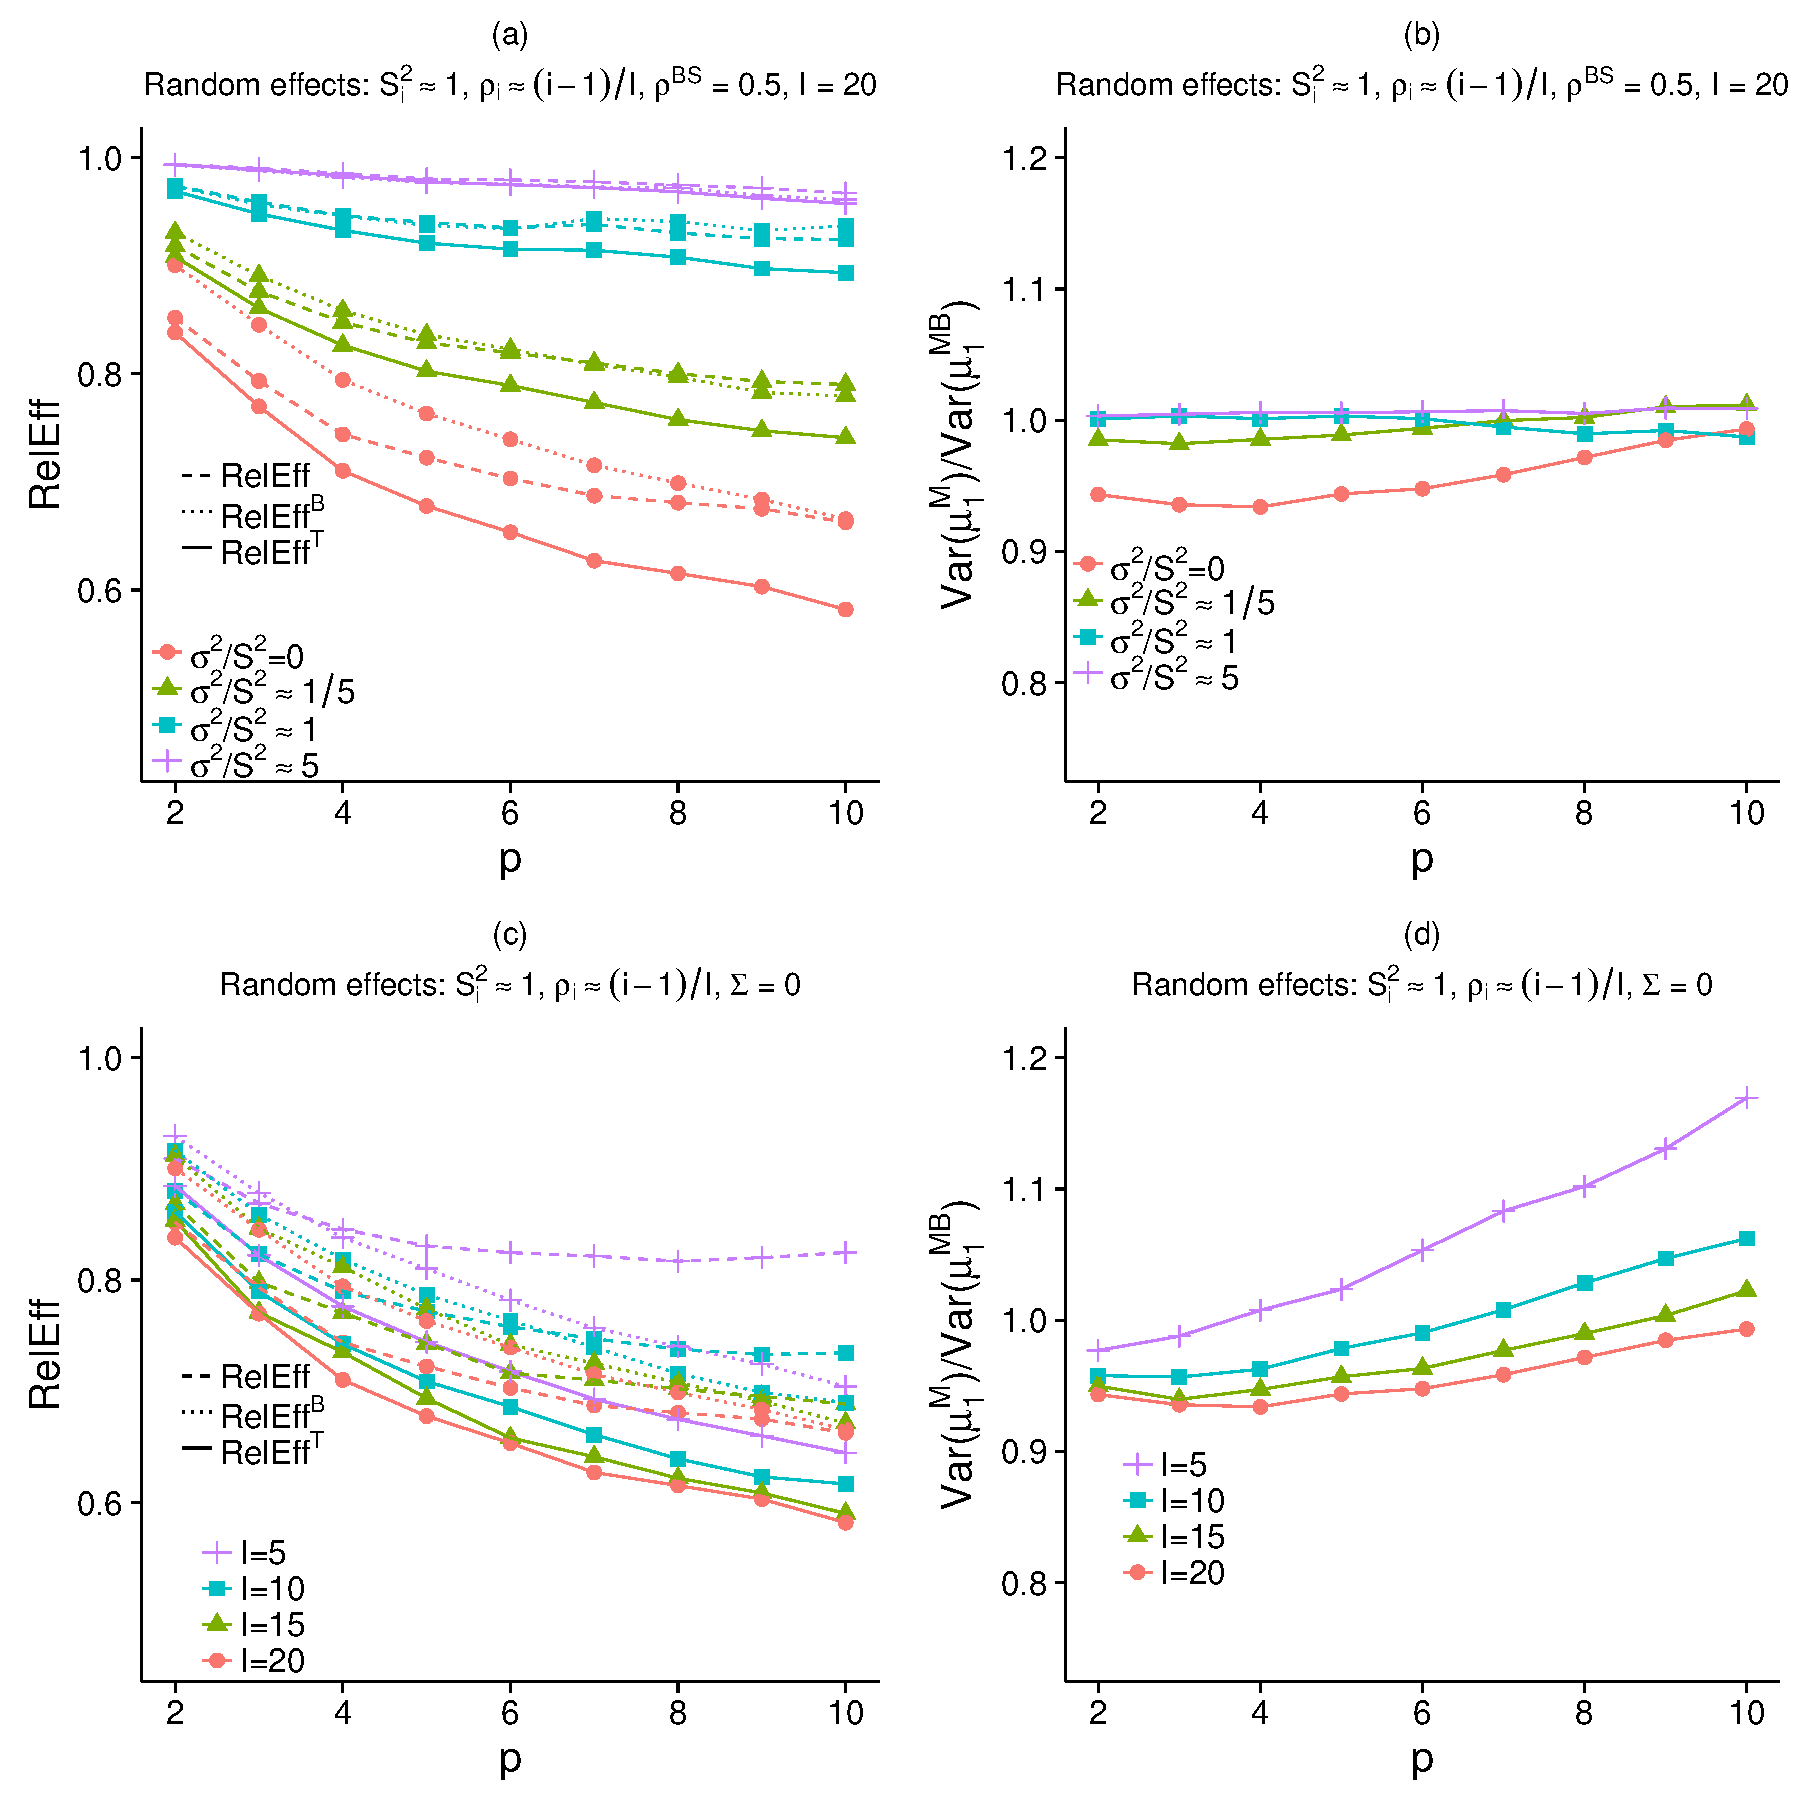
\includegraphics[width=\maxwidth]{figures/Figure_S8_panels_abcd-1} 

}



\end{knitrout}

\end{document}
